\documentclass[german,11pt]{beamer}
% ------------------------------------------------------------------------------
% Packages
\usepackage[german,english,french]{babel}
\usepackage[T1]{fontenc}
\usepackage[utf8]{inputenc}
\usepackage{ragged2e}
\usepackage[normalem]{ulem}


\usepackage{listings}
\usepackage{color}
\usepackage{xcolor} 
\usepackage{plantuml}
% \usepackage{enumitem} \setitemize{leftmargin=*}   // Keine Aufzählung
\usepackage{pgfplots}

\usepackage{csquotes}

\pgfplotsset{compat=1.18}

\definecolor{dkgreen} {rgb}{0,0.6,0}
\definecolor{gray}{rgb}{0.5,0.5,0.5}
\definecolor{mauve}{rgb}{0.58,0,0.82}

\lstset{frame=tb,
  language=Java,
  aboveskip=3mm,
  belowskip=3mm,
  showstringspaces=false,
  columns=flexible,
  basicstyle={\small\ttfamily},
  numbers=none,
  numberstyle=\tiny\color{gray},
  keywordstyle=\color{blue},
  commentstyle=\color{dkgreen},
  stringstyle=\color{mauve},
  breaklines=true,
  breakatwhitespace=true,
  tabsize=3
}
% ------------------------------------------------------------------------------
% Parameters
\mode<presentation>{\usetheme{Luebeck}}
\setbeamertemplate{itemize items}[triangle]
\setbeamercovered{transparent}
\usecolortheme{dove}
\usefonttheme{serif}
\addtobeamertemplate{block begin}{}{\justifying}
% ToC
\AtBeginSection[] {
  \begin{frame}{Inhalt}
    \tableofcontents[currentsection]
  \end{frame}
}
% Headline
\makeatletter
\setbeamertemplate{headline}{%
  \leavevmode%
  \@tempdimb=2.4375ex%
  \ifnum\beamer@subsectionmax<\beamer@sectionmax%
    \multiply\@tempdimb by\beamer@sectionmax%
  \else%
    \multiply\@tempdimb by\beamer@subsectionmax%
  \fi%
  \ifdim\@tempdimb>0pt%
    \advance\@tempdimb by 1.825ex%
    \begin{beamercolorbox}[wd=.5\paperwidth,ht=\@tempdimb]{section in head/foot}%
      \vbox to\@tempdimb{\hfill\insertsectionnavigation{.3\paperwidth}\vfil}%
    \end{beamercolorbox}%
    \begin{beamercolorbox}[wd=.3\paperwidth,ht=\@tempdimb]{subsection in head/foot}%
      \vbox to\@tempdimb{\vfil\insertsubsectionnavigation{.5\paperwidth}\vfil}%
    \end{beamercolorbox}%
    \begin{beamercolorbox}[wd=.2\paperwidth,ht=\@tempdimb]{subsection in head/foot}%
      \vbox to\@tempdimb{\vfil\hfill
\includegraphics[height=1cm]{fig/graphics/logo.jpg}\vfil}
    \end{beamercolorbox}%    
  \fi%
}
\makeatother
% Footline
\makeatletter
\setbeamertemplate{footline}{%
  \leavevmode%
  \hbox{\begin{beamercolorbox}[wd=.5\paperwidth,ht=2.5ex,dp=1.125ex,leftskip=.3cm,rightskip=.3cm]{author in head/foot}%
    \usebeamerfont{author in head/foot}\insertshortdate \hfill \insertshortauthor
  \end{beamercolorbox}%
  \begin{beamercolorbox}[wd=.5\paperwidth,ht=2.5ex,dp=1.125ex,leftskip=.3cm,rightskip=.3cm plus1fil]{title in head/foot}%
    \usebeamerfont{title in head/foot}\insertshorttitle \hfill \insertframenumber\,/\,\inserttotalframenumber
  \end{beamercolorbox}}%
  \vskip0pt%
}
\makeatother

\addto\captionsenglish{% Replace "english" with the language you use
  \renewcommand{\contentsname}%
    {Whatever}%
}

% ------------------------------------------------------------------------------
% Infos
\title[VS]{Verteilte Systeme}
%\subtitle[Short subtitle]{Subtitle}
\author[BCK]{Prof. Dr. Martin Becke}
\date[0.9]{Version 0.9}
\institute[CaDS]{CaDS - HAW Hamburg}
%\logo{
\includegraphics[height=1cm]{fig/graphics/logo.jpg}}
% ------------------------------------------------------------------------------

% Document
\begin{document}

% ------------------------------------------------------------------------------
% Titlepage
\begin{frame}
  \titlepage{}
\end{frame}
% ------------------------------------------------------------------------------
% ToC
%\begin{frame}{Contents}
%  \tableofcontents
%\end{frame}
% ------------------------------------------------------------------------------
 
\section{Architekturparadigmen}
%\subsection{Einleitung}
\begin{frame}
  \frametitle{Architekturparadigmen}
  \framesubtitle{Überblick}
  \begin{itemize}
    \item Schichtenarchitektur
    \item Client-Server-Architektur
    \item Service-Orientierte Architektur (SOA)
    \item Ereignisgesteuerte Architektur (Event-Driven)
    \item Microservices-Architektur
    \item Peer-to-Peer-Architektur (P2P)
  \end{itemize}
\end{frame}

\begin{frame}
  \frametitle{Architekturparadigmen}
  \framesubtitle{Grundelement node}
  \begin{itemize}
    \item Autonomes Computerelement
    \item Hardware-Systeme oder Software-Prozesse
    \item Teilen keinen gemeinsamen Speicher
    \item Kommunikation über Nachrichten 
  \end{itemize}
\end{frame}
%\section{Einleitung}
\subsection{Schichtenarchitektur}
\begin{frame}
  \frametitle{Schichtenarchitektur}
  \framesubtitle{Definition}
  \begin{itemize}
    \item Hierarchische Struktur 
    \item Definiert Abstraktionsebenen mit allgemeinen Schnittstellen
    \item Jede Schicht repräsentiert ein Set von Funktionen
    \item Jede Schicht hat eine oder mehrere Interpretationen
    \item Jede Interpretation implementiert Protokolle 
  \end{itemize}
\end{frame}
\begin{frame}
  \frametitle{Schichtenarchitektur}
  \framesubtitle{Bedeutung}
  \begin{itemize}
    \item Komplexe Systeme in kleinere, einfachere Teile zerlegen
    \item Trennung von Verantwortlichkeiten 
    \item Schichten können unabhängig entwickelt, getestet und gewartet werden
    \item Jede Schicht kann als Komponente verstanden werden
    \item Interoperabilität und Kompatibilität steigt
    \item Wiederverwendbarkeit steigt 
    \item Chance und Risiko für Sicherheit
    \item Historisch wichtig und immer noch hohen Einfluss
  \end{itemize}
\end{frame}
\begin{frame}
  \frametitle{Schichtenarchitektur}
  \framesubtitle{Beispiele}
  \begin{itemize}
    \item ISO OSI Referenzmodell
    \item DECnet
    \item Cloud Architekturen
    \item Micro Service Architekturen
  \end{itemize}
\end{frame}

\begin{frame}
  \frametitle{Layer}
  \framesubtitle{Definition}
  \begin{itemize}
    \item Logische Gruppierung von Funktionen
    \item Schichten werden in der Regel vertikal angeordnet
    \item Jede Schicht erfüllt eine spezifische Funktion
  \end{itemize}
\end{frame}

\begin{frame}
  \frametitle{Layer}
  \framesubtitle{Beispiel}
  \begin{itemize}
    \item Presentation Layer
    \item Business Logic Layer
    \item Data Access Layer
  \end{itemize}
\end{frame}


\begin{frame}
  \frametitle{Layer}
  \framesubtitle{Als Komponenten}
  \begin{figure}[!h]
    \centering
    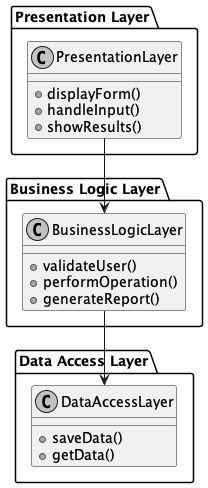
\includegraphics[width=0.20\textwidth]{fig/uml/simple-layers.png}
    \caption{Einfaches Schichtenmodell}
    \label{fig:simple-layer}
  \end{figure}
\end{frame}

\begin{frame}
  \frametitle{Tier}
  \framesubtitle{Definition}
  \begin{itemize}
    \item Physische oder logische Aufteilung
    \item Jedes Tier hat normalerweise eine spezifische Funktion 
    \item Normalerweise durch eine Netzwerkverbindung miteinander verbunden
  \end{itemize}
\end{frame}

\begin{frame}
  \frametitle{Tier}
  \framesubtitle{Beispiel}
  \begin{itemize}
    \item Präsentations-Tier
    \item Anwendungs-Tier 
    \item Datenbank-Tier
  \end{itemize}
\end{frame}

\begin{frame}
  \frametitle{Tier}
  \framesubtitle{Als Komponenten}

  \begin{figure}[!h]
    \centering
    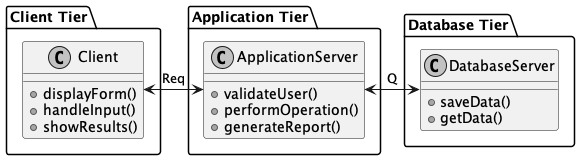
\includegraphics[width=0.95\textwidth]{fig/uml/simple-tiers.png}
    \caption{Einfaches Tier Modell}
    \label{fig:simple-tier}
  \end{figure}
\end{frame}
%\section{Einleitung}
\subsection{Single Node (Application0)}
\begin{frame}
  \frametitle{Single Node }
  \framesubtitle{Definition}
  \begin{itemize}
    \item Architekturtyp
    \item Anwendungen werden auf einem einzelnen Knoten ausgeführt
    \item Keine Verteilung der Funktionen
    \item Knoten kann ein physischer Server oder eine virtuelle Maschine sein
    \item Knoten kann von verschiedenen Systemen sammeln und verarbeiten
  \end{itemize}
\end{frame}

\begin{frame}
  \frametitle{Single Node }
  \framesubtitle{Vorteile}
  \begin{itemize}
    \item Entwicklung und Testen
    \item Kleine Anwendungen
    \item Datenintensive Anwendungen
  \end{itemize}
\end{frame}

\begin{frame}
  \frametitle{Single Node }
  \framesubtitle{Umsetzung und Beispiele}
  \begin{itemize}
    \item Container-Technologien
    \item Serverless-Computing (AWS Lambda)
    \item Netflix: Netflix verwendet das Single-Node-Pattern, um die Datenverarbeitung in ihren AWS-Cloud-Instanzen
    \item Airbnb: Airbnb verwendet das Single-Node-Pattern, um ihre Webanwendung (nicht die Daten) in einem einzigen Knoten zu hosten
  \end{itemize}
\end{frame}
%\section{Einleitung}
\subsection{Overlay Network}
\begin{frame}
  \frametitle{Overlay}
  \framesubtitle{Idee}
  \begin{itemize}
    \item Logische Verbindung muss keiner physikalischen Verbindung entsprechen
    \item Genutzte Netzwerkstruktur besteht häufig auf der obersten Schicht einer physikalischen Netzwerkstruktur
    \item Zusätzliche Abstraktion und Organisation
    \item Zusätzliche Komplexität und Overhead
  \end{itemize}
\end{frame}

\begin{frame}
  \frametitle{Overlay}
  \framesubtitle{Beispiel P2P}
  \begin{itemize}
    \item In einem P2P-Netzwerk sind die Knoten gleichberechtigte Teilnehmer
    \item Teil oder voll vermascht 
    \item Bekanntes Beispiel für ein P2P-Overlay-Netzwerk ist BitTorrent
  \end{itemize}
\end{frame}

\begin{frame}
  \frametitle{Overlay}
  \framesubtitle{P2P - Strukturierte Netzwerke}
  \begin{itemize}
    \item Geordnete Struktur
    \item Verwenden meist deterministische Verfahren oder Algorithmen
    \item Routing effizienter und vorhersagbarer 
    \item Ein Beispiel für ein strukturiertes Routing-Verfahren ist DHT
    \item Suche kann in logarithmischer Zeit (O(log N)) durchgeführt werden
  \end{itemize}
\end{frame}

\begin{frame}
  \frametitle{Overlay}
  \framesubtitle{P2P - Un-Strukturierte Netzwerke}
  \begin{itemize}
    \item Keine Struktur
    \item Verwendung auf Basis von Heuristiken und Zufall
    \item Routing kaum effizient zu gestalten 
    \item Typisch ist hohe Netzwerklast
    \item Flooding- oder Random-Walk-Verfahren für die Suche
    \item Schädliche Teilnehmer ein besonderes Problem
  \end{itemize}
\end{frame}
%\section{Einleitung}
\subsection{Middleware Architektur}
\begin{frame}
  \frametitle{Middleware Architektur}
  \framesubtitle{Idee}
  \begin{itemize}
    \item Kapselung der Aufgabe
    \item Eigene Schicht für die Herausforderung der verteilten Systemen 
    \item Schicht wird als \enquote{Middleware-}Schicht bezeichnet
    \item Bietet im besten Fall die Schnittstelle des kohärenten Systems
  \end{itemize}
\end{frame}

\begin{frame}
  \frametitle{Middleware Architektur}
  \framesubtitle{Definition nach Tanenbaum}
  \begin{itemize}
    \item Bereitstellung eines breiten Angebotes für die Kommunikation
    \item Dem (Un-)Marshaling Prozess 
    \item Protokolle zur Namensauflösung
    \item Sicherheitsprotokolle
    \item Mechanismen zur Steigerung der Skalierung
  \end{itemize}
\end{frame}

\begin{frame}
  \frametitle{Middleware Architektur}
  \framesubtitle{Erweiterte Anforderungen}
  \begin{itemize}
    \item Mehrere Sprachen
    \item Mehreren Betriebssystemen und Hardwaretypen
    \item Mehrere Netzwerkprotokolle zur Einbindung von Internetstrukturen
  \end{itemize}
\end{frame}

\begin{frame}
  \frametitle{Middleware Architektur}
  \framesubtitle{Kommunikation}
  \begin{itemize}
    \item Point to point
    \item Point to multipoint
    \item Publish/subscribe
    \item Client/Server, Request/Reply
    \item Mobile code
    \item Virtual shared
  \end{itemize}
\end{frame}

\begin{frame}
  \frametitle{Middleware Architektur}
  \framesubtitle{Message Oriented Middleware (MOM)}
  \begin{itemize}
      \item Direkte Kommunikation zwischen Anwendungen (Message Passing)
      \item Indirekte Kommunikation über eine Warteschlange (Message Queueing)
      \item Herausgeber stellt dem Abonnenten Nachrichten zur Verfügung (Publish \& Subscribe)
  \end{itemize}
\end{frame}


%\section{Einleitung}
\subsection{Client-Server-Architektur}
\begin{frame}
  \frametitle{Client-Server-Architektur}
  \framesubtitle{Modell}
  \begin{itemize}
    \item In dieser Architektur gibt es zwei Hauptkomponenten
    \item Client - nutzt (Consumer)
    \item Server - bietet an (Provider)
    \item Ein spezielle \enquote{2-Tier Architektur}
    \item Front-End-Client und einem Back-End-Server
  \end{itemize}
\end{frame}

\begin{frame}
  \frametitle{Client-Server-Architektur}
  \framesubtitle{Beispiele}
  \begin{itemize}
    \item Webanwendungen
    \item Datenbankanwendungen
  \end{itemize}
\end{frame}

\begin{frame}
  \frametitle{Client-Server-Architektur}
  \framesubtitle{Kaskadenartige Kommunikation}
  \begin{itemize}
    \item n-Tier-Architektur sind Tiers sowohl Consumer- als auch Provider
    \item Auswirkung auf Latenz, Komplexität, Fehleranfälligkeit, Skalierbarkeit
    \item Einführung von Optimierungsmechanismen, wie Caching, Lastverteilung, asynchrone Kommunikation 
  \end{itemize}
\end{frame}

\begin{frame}
  \frametitle{Client-Server-Architektur}
  \framesubtitle{SSP - Stub/Skeleton Chains}
  \begin{itemize}
    \item Eine Implementierungsform von Interface-Definitionen zur Kommunikation
    \item Methodenaufrufe von einer Schicht zur anderen
    \item Stub ist ein Platzhalter für eine entfernte Methode (Lokal oder Remote)
    \item SSP Stub/Skeleton Chains sind eine Sequenz von Stubs und Skeletons
    \item Gemeinsame Sprache zwischen verschiedenen Schichten oder Tiers
  \end{itemize}
\end{frame}
%\section{Einleitung}
\subsection{Event-Driven Architektur}
\begin{frame}
  \frametitle{Event-Driven Architecture}
  \framesubtitle{Idee}
  \begin{itemize}
    \item Kommunikation getrieben über Events oder Nachrichten
    \item Komponenten reagieren auf Events oder Nachrichten
    \item Keine direkte Kommunikation (Vergleich Eventbus)
  \end{itemize}
\end{frame}

\begin{frame}
  \frametitle{Event-Driven Architecture}
  \framesubtitle{Beispiele}
  \begin{itemize}
    \item Aktienhandelssystem
    \item IoT-Sensornetzwerk
    \item E-Commerce-Plattform
  \end{itemize}
\end{frame}

\begin{frame}
  \frametitle{Event-Driven Architecture}
  \framesubtitle{Aufbau}
  \begin{itemize}
    \item Event-Producer
    \item Event-Channel
    \item Event-Consumer
  \end{itemize}
\end{frame}

\begin{frame}
  \frametitle{Event-Driven Architecture}
  \framesubtitle{Erweiterung um Lambda Architecture}
  \begin{itemize}
    \item Häufig im Kontext von Big-Data- und Echtzeitanalysen
    \item Datenverarbeitungsarchitekturmuster
    \item Latenzarme und fehlertolerante Analyse- und Verarbeitungssysteme
  \end{itemize}
\end{frame}

\begin{frame}
  \frametitle{Lambda Architecture}
  \framesubtitle{Aufbau}
  \begin{itemize}
    \item Batch-Layer
    \item Speed-Layer
    \item Serving-Layer
  \end{itemize}
\end{frame}



%\section{Einleitung}
\subsection{Microservices-Architektur}
\begin{frame}
  \frametitle{Microservices-Architektur}
  \framesubtitle{Idee}
  \begin{itemize}
    \item Anwendung ist Sammlung kleiner, unabhängiger und modularer Dienste 
    \item Dienste sind lose gekoppelt, können unabhängig voneinander entwickelt, bereitgestellt und skaliert werden
    \item Entwicklerteam je Dienst
    \item Erhöhte Komplexität, Kommunikations-Overhead, Sicherheits- und Authentifizierungsfragen
  \end{itemize}
\end{frame}

\begin{frame}
  \frametitle{Microservices-Architektur}
  \framesubtitle{Beispiele}
  \begin{itemize}
    \item Online-Shop
    \item Content-Management-System
    \item Bankanwendung
  \end{itemize}
\end{frame}
%\section{Einleitung}
\subsection{Peer-to-Peer-Architektur}
\begin{frame}
  \frametitle{Peer-to-Peer-Architektur}
  \framesubtitle{Idee}
  \begin{itemize}
    \item Einzelne Knoten (Peers) kommunizieren direkt miteinander 
    \item Knoten sowohl Clients als auch Server
    \item Teilen Ressourcen und tragen gemeinsam zur Leistung und Skalierbarkeit des Netzwerks bei
  \end{itemize}
\end{frame}
\begin{frame}
  \frametitle{Peer-to-Peer-Architektur}
  \framesubtitle{Beispiele}
  \begin{itemize}
    \item Dateifreigabe
    \item Kommunikation und Messaging
    \item Blockchain und Kryptowährungen
    \item Beispiel wird nochmals Overlay und P2P Architektur deutlich machen
  \end{itemize}
\end{frame}
%\section{Einleitung}
\subsection{Hexagonal Onion Architektur}
\begin{frame}
  \frametitle{Hexagonal Onion Architektur}
  \framesubtitle{Idee}
  \begin{itemize}
    \item Kombination aus zwei bekannten Architekturmustern: Hexagonale Architektur und Zwiebelarchitektur
    \item Die Kernlogik des Systems ist unabhängig von externen Einflüssen 
    \item Ports und Adaptern dienen als Schnittstelle zwischen der Kernlogik und externen Anliegen
  \end{itemize}
\end{frame}

\begin{frame}
  \frametitle{Hexagonal Onion Architecture}
  \framesubtitle{Typische Schichten}
  \begin{itemize}
    \item Domain
    \item Application 
    \item Ports
    \item Adapters
  \end{itemize}
\end{frame}

\begin{frame}
  \frametitle{Hexagonal Onion Architecture}
  \framesubtitle{Beispiel mit Microservices}
  \begin{itemize}
    \item Domain: Verwalten von Produkten und Dienstleister
    \item Application: Prozesse für Kauf, Verkauf, Retoure, Wartung, etc 
    \item Microservice: Online Bestellungs-Service mit Abhängigkeit Bezahlservice
    \item Microservice: Online Produkt-Service
    \item Microservice: Online Zahlungs-Service
    \item Microservice: Online Versand-Service 
  \end{itemize}
\end{frame}
%\section{}
\subsection{Time vs Event Triggered}
\begin{frame}
  \frametitle{Time Triggered vs Event Triggered}
  \framesubtitle{Diskussion}
  \begin{itemize}
    \item Synchronisation
    \item Determinismus
    \item Koordination
    \item Latenz
    \item Ressourcen 
  \end{itemize}
\end{frame}

% ------------------------------------------------------------------------------
% Fin
\end{document}